\documentclass[10pt,a4paper]{article}
\usepackage[T1]{fontenc}
\usepackage[utf8]{inputenc}
\usepackage{lmodern}
\usepackage[margin=0.6in]{geometry}
\usepackage{xcolor}
\usepackage{tikz}
\usepackage{tabularx}
\usepackage{booktabs}
\usepackage{array}
\usepackage{enumitem}
\usepackage{fontawesome} 
\usetikzlibrary{arrows.meta,positioning,fit,backgrounds,calc,shapes.multipart,shadows}

\definecolor{branddark}{HTML}{0F172A}
\definecolor{brandslate}{HTML}{334155}
\definecolor{brandblue}{HTML}{2563EB}
\definecolor{boxfill}{HTML}{F8FAFC}
\definecolor{boxline}{HTML}{94A3B8}

\definecolor{vibrantgreen}{HTML}{34D399}
\definecolor{vibrantblue}{HTML}{38BDF8}
\definecolor{vibrantamber}{HTML}{FBBF24}
\definecolor{vibrantred}{HTML}{FB7185}
\definecolor{vibrantviolet}{HTML}{A78BFA}

\pagestyle{empty}
\setlength{\parindent}{0pt}
\setlength{\parskip}{2pt}
\renewcommand{\arraystretch}{1.2}

\tikzset{
  basebox/.style={
    rounded corners=6pt,
    draw=branddark,
    line width=0.9pt,
    align=center,
    font=\footnotesize,
    inner sep=6pt,
    drop shadow={shadow xshift=1.5pt, shadow yshift=-1.5pt, opacity=0.12}
  },
  titlebox/.style={
    basebox,
    fill=brandslate!15,
    font=\bfseries\normalsize,
    text width=\textwidth-16pt,
    minimum height=0.7cm,
    align=left
  },
  metricbox/.style={
    basebox,
    fill=white,
    text width=4.8cm,
    minimum height=1.2cm,
    align=center
  }
}

\begin{document}

{\LARGE\bfseries \textnormal{\faLineChart}\ Business Impact \& ROI Model}\\[2mm]
{\large AgriAdvisor Local Fallback Engine (Small-Scale Deployment Projection)}

\vspace{2mm}
\hrule
\vspace{4mm}

\noindent
\begin{tikzpicture}
  \node[titlebox] (assumptions) {\textnormal{\faCogs}\ \textbf{1. Baseline Metrics \& Core Assumptions (Monthly Run-Rate)}};
\end{tikzpicture}
\vspace{1mm}

\begin{itemize}[leftmargin=*, label=\textcolor{brandblue}{\textnormal{\faLeaf}}, itemsep=2pt]
    \item \textbf{System Drop Rate:} Approximately 250 queries drop per month due to rural network timeouts.
    \item \textbf{Manual Recovery Cost:} Support agents must call back farmers to resolve dropped queries.
    \item \textbf{Time \& Labor:} Each manual callback takes an average of 12 minutes.
    \item \textbf{Labor Rate:} Fully loaded cost of a tier-1 support agent is \textnormal{\faInr} 150 per hour.
    \item \textbf{Fallback Efficiency:} The local offline reasoning engine successfully answers 80\% of dropped queries natively.
    \item \textbf{Customer Value:} Average Revenue Per User (ARPU) is \textnormal{\faInr} 50/month. Unanswered drops have a 20\% churn risk.
\end{itemize}

\vspace{4mm}

\noindent

\begin{tikzpicture}
  \node[titlebox] (savings) {\textnormal{\faClockO}\ \textbf{2. Operational Cost Savings (Time \& Labor)}};
\end{tikzpicture}
\vspace{1mm}

\begin{tabularx}{\textwidth}{>{\raggedright\arraybackslash\bfseries}p{4cm} X >{\raggedright\arraybackslash\bfseries}p{3cm}}
\toprule
Metric & \normalfont\textbf{Calculation Logic} & Impact \\
\midrule
Total Manual Time Avoided & 250 drops $\times$ 80\% handled locally $\times$ 12 mins per resolution & 40 Hours / mo \\
\addlinespace
Labor Cost Reduced & 40 hours saved $\times$ \textnormal{\faInr} 150 per hour & \textnormal{\faInr} 6,000 / mo \\
\addlinespace
API Costs Avoided & 200 fallback queries rerouted from cloud LLM & Negligible \\
\bottomrule
\end{tabularx}

\vspace{4mm}

\noindent

\begin{tikzpicture}
  \node[titlebox] (revenue) {\textnormal{\faShield}\ \textbf{3. Revenue Retention \& Risk Mitigation}};
\end{tikzpicture}
\vspace{1mm}

\begin{tabularx}{\textwidth}{>{\raggedright\arraybackslash\bfseries}p{4cm} X >{\raggedright\arraybackslash\bfseries}p{3cm}}
\toprule
Metric & \normalfont\textbf{Calculation Logic} & Impact \\
\midrule
Churn Events Prevented & 200 local resolutions $\times$ 20\% risk of churn if left unanswered & 40 Users Retained \\
\addlinespace
Monthly Revenue Protected & 40 retained users $\times$ \textnormal{\faInr} 50 ARPU & \textnormal{\faInr} 2,000 / mo \\
\bottomrule
\end{tabularx}

\vspace{6mm}

\noindent

\begin{tikzpicture}
  \node[titlebox, fill=brandblue!10, draw=brandblue] (totals) {\textnormal{\faTrophy}\ \textbf{4. Total Quantified Business Impact}};
\end{tikzpicture}
\vspace{3mm}

\noindent
\makebox[\textwidth][c]{
\begin{tikzpicture}
  \node[metricbox, draw=vibrantamber] (monthly) at (0,0) {
    \textcolor{brandslate}{\textbf{Total Monthly Impact}}\\[1.5mm]
    {\Large\bfseries \textnormal{\faInr} 8,000}
  };
  
  \node[metricbox, draw=vibrantgreen] (annual) at (5.5,0) {
    \textcolor{brandslate}{\textbf{Projected Annual ROI}}\\[1.5mm]
    {\Large\bfseries \textnormal{\faInr} 96,000}
  };

  \node[metricbox, draw=brandblue] (capacity) at (11,0) {
    \textcolor{brandslate}{\textbf{Support Capacity Freed}}\\[1.5mm]
    {\Large\bfseries 480 Hours/yr}
  };
\end{tikzpicture}
}

\vspace{6mm}

\noindent

\begin{tikzpicture}
  \node[titlebox] (intangible) {\textnormal{\faHeartbeat}\ \textbf{5. Qualitative \& Strategic Benefits}};
\end{tikzpicture}
\vspace{1mm}

\begin{itemize}[leftmargin=*, label=\textcolor{brandblue}{\textnormal{\faCheck}}, itemsep=2pt]
    \item \textbf{Farmer Trust \& Reliability:} Providing instant answers even in zero-network zones builds high brand loyalty and reliance on the AgriAdvisor platform.
    \item \textbf{Support Team Mental Bandwidth:} Removes highly repetitive, low-tier follow-up calls from the support queue, allowing agents to focus on complex agronomy escalations.
    \item \textbf{Graceful Degradation:} System degrades from "Cloud Intelligence" to "Local Intelligence" rather than showing an error screen, vastly improving the UX.
\end{itemize}

\end{document}